\chapter{Umsetzung}
\label{cha:Umsetzung}

\section{Umsetzung der MVVM-Struktur}
Die Anwendung wurde überwiegend nach dem Model-View-ViewModel-(MVVM)-Entwurfsmuster umgesetzt. Sie gliedert sich in die fünf Schichten Views, View-Models, Models, Services und Repositories.
\subsection{View}
Die Views bilden die Benutzeroberfläche der Anwendung. Sie enthalten ausschließlich die Definition und Darstellung der grafischen Elemente sowie die notwendige Datenbindung zu den jeweiligen View-Models. Dabei gibt es eine Main-View, die sich rein um die Navigation zwischen verschiedenen Reitern kümmert. Außerdem sind auf ihr verschiedene Informationen dargestellt, die unabhängig vom aktuell ausgewählten Reiter permanent sichtbar sein sollen. 

Der eigentliche Inhalt der einzelnen Reiter wird innerhalb eines \lstinline|ContentControl|-Elements angezeigt. Durch den Austausch des aktuell zugewiesenen Inhalts können verschiedene Ansichten dynamisch geladen werden.

Für jeden Reiter, der in dem \lstinline|ContentControl|-Feld angezeigt werden soll, gibt es eine eigene View als Benutzersteuerelement. Im Listing \ref{lst:MessageView} sieht man vereinfacht den XAML-Code für die Nachrichtentabelle. Dabei wird über ein Binding die \textit{ObservableCollection} \lstinline|Messages| als Datengrundlage für die Nachrichtentabelle verknüpft.
Ändert sich in der View das in der Tabelle ausgewählte Objekt, wird durch die Datenbindung mit der Variable \lstinline|SelectedItem| diese automatisch auch überschrieben. In der kompakten Ansicht kann daraufhin der Payload für das ausgewählte Objekt in der Tabelle angepasst werden. Die einzelnen Spalten verknüpfen sich mit den einzelnen Objekten der in \lstinline|Messages| gespeicherten Nachrichtenmodelle.
Dadurch entsteht eine Tabelle, die automatisch die einzelnen in \lstinline|Messages| gespeicherten Nachrichten anzeigt.
\begin{lstlisting}[
    language={[Sharp]C},
    caption={Programmcode für MQTT-Verbindung},
    label={lst:MessageView}
    ]
<DataGrid ItemsSource="{Binding Messages}"
          SelectedItem="{Binding SelectedItem}"
          AutoGenerateColumns="False"
          IsReadOnly="True">
    <DataGrid.Columns>
        <DataGridTextColumn Header="ID"
                            Binding="{Binding Id}"/>
        <DataGridTextColumn Header="Sender"
                            Binding="{Binding Sender}"/>
        <DataGridTextColumn Header="Zeit"
                            Binding="{Binding Timestamp}"/>
        <DataGridTextColumn Header="Topic"
                            Binding="{Binding Topic}"/>
        <DataGridTemplateColumn Header="Payload">
            <DataGridTemplateColumn.CellTemplate>
                <DataTemplate>
                    <TextBlock Text="{Binding Payload}"
                               TextWrapping="Wrap"/>
                </DataTemplate>
            </DataGridTemplateColumn.CellTemplate>
        </DataGridTemplateColumn>
    </DataGrid.Columns>
</DataGrid>
\end{lstlisting}

\subsection{View-Model}
Die View-Models bilden die Verbindung zwischen der Benutzeroberfläche und der Anwendungslogik. Sie stellen der View die notwendigen Daten aus den Models, aber auch aus den Service- und Repository-Dateien zur Verfügung und reagieren auf Benutzereingaben. Dabei enthalten sie keine beziehungsweise so wenig  Informationen  wie möglich über die konkrete Darstellung der Benutzeroberfläche.

Die einzelnen View-Models verwalten beispielsweise die angezeigten Nachrichten, die Teilnehmerliste oder die Verbindungsinformationen. Änderungen an den Daten werden über \textit{ObservableCollections} und \textit{ObservableProperties} automatisch an die View weitergegeben \autocite{sergio0694EinfuehrungMVVMToolkitCommunity}. Dadurch aktualisiert sich die Benutzeroberfläche ohne zusätzlichen Programmcode.
Durch den Einsatz von \textit{ObservableCollections} werden Änderungen automatisch an die Benutzeroberfläche übertragen. Dies reduziert den Implementierungsaufwand erheblich und vereinfacht die Datenbindung. Gleichzeitig führt jede Änderung zu einer Benachrichtigung der Oberfläche, wodurch bei sehr großen Datenmengen zusätzliche Last auf dem UI-Thread entstehen kann.

Darüber hinaus sind die View-Models für die Navigation zwischen den einzelnen Ansichten zuständig und koordinieren die Kommunikation mit den Services. Die eigentliche Geschäftslogik wird jedoch nicht in den View-Models implementiert, sondern an die entsprechenden Services delegiert.
\subsection{Models}
Die Models stellen die Struktur der Daten dar, die von den Services an die View-Models weitergegeben werden. Sie beschreiben dabei die Eigenschaften der verschiedenen Objekte, beispielsweise Nachrichten, Teilnehmer, Einstellungen oder Zustandsverläufe. 

Die Model-Klassen enthalten dabei ausschließlich die benötigten Datenfelder und keine Logik zur Darstellung oder Verarbeitung der Daten. Durch diese Trennung bleibt die Anwendung übersichtlich und die einzelnen Komponenten können unabhängig voneinander erweitert werden.
\subsection{Services}
Die Services enthalten die Geschäftslogik der Anwendung. Sie verarbeiten eingehende MQTT-Nachrichten, analysieren deren Inhalt und bereiten die Daten für die weitere Verwendung auf. 

Durch die Auslagerung der Geschäftslogik aus den View-Models bleiben die View-Models übersichtlich und konzentrieren sich auf ihre eigentliche Aufgabe, die Bereitstellung der Daten für die Benutzeroberfläche.
\subsection{Repositories}
Die Repositories sind für die Speicherung beziehungsweise das Laden von Daten aus der SQLite-Datenbank zuständig und bilden somit die Schnittstelle zwischen der Anwendungslogik und der Datenbank. 

Für die verschiedenen Datenbereiche existieren eigene Repository-Klassen, beispielsweise für Nachrichten, Teilnehmer, Fehler oder Einstellungen. Für jede dieser Bereiche werden von den Repositories eigene Tabellen in der Datenbank angelegt und Methoden zur Aktualisierung, zum Laden und zur Speicherung von Daten implementiert.

Diese Trennung verbessert die Wartbarkeit des Programms erheblich, da Änderungen an der Datenhaltung ausschließlich innerhalb der jeweiligen Repository-Klasse vorgenommen werden müssen. Gleichzeitig wird die Wiederverwendbarkeit von Datenzugriffen drastisch erhöht.
\section{MQTT-Kommunikation}
\subsection{Verbindungsaufbau}
Für die Verbindung, aber auch später für das Empfangen und Senden von Nachrichten, wird eine Referenz auf einen MQTT-Client benötigt. Dazu besitzt die ,,MQTTnet''-Bibliothek das Interface ,,IMqttClient''. In der Klasse \texttt{MqttService} wird eine Instanz des MQTT-Clients  in der Variable \lstinline|Client| des Typs \lstinline|IMqttClient| gespeichert. 
Diese repräsentiert den MQTT-Client der Anwendung und dient als zentrale Schnittstelle für die Kommunikation mit dem Broker.
 
Der Verbindungsaufbau mit einem MQTT-Broker wird mithilfe der ,,MQTTnet''-Bibliothek implementiert. Wie in Listing \ref{lst:MQTT-Connection} zu erkennen ist, werden der Methode die Zeichenketten ,,Broker-IP'' und ,,Broker-Port'' sowie ,,Username'' und ,,Passwort'' übergeben. 
Mithilfe des sogenannten Optionsbuilders aus der ,,MQTTnet''-Bibliothek werden die Optionen für die Verbindung erstellt. Die Verbindung zum Broker wird anschließend durch den Aufruf von \lstinline| Client.ConnectAsync(options)| hergestellt. 
\begin{lstlisting}[
    language={[Sharp]C},
    caption={Programmcode für MQTT-Verbindung},
    label={lst:MQTT-Connection}
    ]
public async Task<bool> Connect(string brokerip, string port, string username, string password, string topic="#")
{
    bool connected = false;

    try
    {

        int brokerPort = int.Parse(port);

        var optionsBuilder = new MqttClientOptionsBuilder()
            .WithTcpServer(brokerip, brokerPort);

        if (!string.IsNullOrWhiteSpace(username) &&
            !string.IsNullOrWhiteSpace(password))
        {
            optionsBuilder.WithCredentials(username, password);
        }

        var options = optionsBuilder.Build();

        var cts = new CancellationTokenSource(TimeSpan.FromSeconds(3));

        await Client.ConnectAsync(options, cts.Token);
        await Client.SubscribeAsync(topic);
        connected = true;
    }
    catch (OperationCanceledException)
    {
        connected = false;
    }
    catch (Exception ex)
    {
        connected = false;
    }
    return connected;
}
\end{lstlisting}

Um die Verbindung zum Broker wieder zu trennen, wird die Methode \lstinline|Disconnect()| implementiert. In dieser wird zum einen die Verbindung durch  den Befehl \lstinline|Client.DisconnectAsync| getrennt. Zum anderen müssen die abonnierten Topics wieder abbestellt werden. 
Das geschieht durch den Befehl \lstinline|Client.UnsubscribeAsync| . Werden die Topics nicht wieder abbestellt werden diese bei einem erneuten Verbindungsaufbau mehrfach abonniert, wodurch eingehende Nachrichten mehrfach empfangen und angezeigt werden.
\begin{lstlisting}[
    language={[Sharp]C},
    caption={Event und Eventhandler zum Erkennen von Verbindungsverlusten},
    label={lst:disconnected}
    ]
Client.DisconnectedAsync += async e =>
{
    Disconnected?.Invoke();
    await Client.UnsubscribeAsync(topic);
};
\end{lstlisting}


Neben dem manuellen Verbinden und Trennen mit dem Broker muss die Anwendung auch erkennen können, ob die Verbindung zum Broker möglicherweise verloren ging. ,,MQTTnet'' stellt hierfür das Event \lstinline|DisconnectedAsync| bereit, das bei einem Verbindungsverlust ausgelöst wird. Wie im Listing \ref{lst:disconnected} zu sehen ist, 
wird im zugehörigen Eventhandler erneut ein weiteres Event ausgelöst, das die Informationen an das Main-View-Model und von da an die UI überträgt. Außerdem werden hier durch \lstinline|Client.UnsubscribeAsync(topic)| die Topics abbestellt.
\subsection{Empfangen von Nachrichten}
Für das Empfangen der Nachrichten werden alle Topics durch den Befehl \lstinline|Client.SubscribeAsync(topic)| abonniert. Die Variable ,,topic'', auf die die Methode zugreift, ist dabei ein String und enthält ,,\#'', was eine sogenannte Wildcard für alle Topics ist. 
Damit andere Dateien beziehungsweise Programmabschnitte auf die empfangenen Nachrichten zugreifen können, wird ein Event erstellt, der bei Nachrichtenempfang automatisch aufgerufen wird (siehe Listing \ref{lst:ReceivedMessages}). Dafür stellt ,,MQTTnet'' das Event \lstinline|ApplicationMessageReceivedAsync| bereit.  
In dessen Eventhandler wird das Topic der Nachricht in einer Stringvariable gespeichert, während die binären Payload-Daten zunächst dekodiert und anschließend als String gespeichert werden. Zum Schluss wird innerhalb dieses Eventhandlers das Event \lstinline|MessageReceived| aufgerufen und beide Variablen an das Event übergeben.
\begin{lstlisting}[
    language={[Sharp]C},
    caption={Event und Eventhandler zum Erkennen des Eintreffens von Nachrichten},
    label={lst:ReceivedMessages}
    ]
Client.ApplicationMessageReceivedAsync += e =>
{
    string receivedTopic = e.ApplicationMessage.Topic;
    string receivedPayload = Encoding.UTF8.GetString(e.ApplicationMessage.Payload);
    MessageReceived?.Invoke(receivedTopic, receivedPayload);
    return Task.CompletedTask;
};
\end{lstlisting}

Der Service, der für das Speichern und Laden von Nachrichten zuständig ist, abonniert das \lstinline|MessageReceived| Event und registriert einen Eventhandler.  Der Eventhandler ruft die in Listing \ref{lst:AddNewMessages} gezeigte Methode \lstinline|async Task AddNewMessage()| auf.
Diese parst die empfangene Payload als JSON und gibt den in der Payload beschriebenen Sender der Nachricht aus.  Der Sender der Nachricht steht unter ,,host'' in ,,messageSource'' im sogenannten Header der Nachricht. Anschließend übergibt die Methode den Sender, Topic und die Payload an die Methode \lstinline|AddMessage| von ,,MessagesRepo''.
Dadurch wird die Nachricht mit aufsteigender Identifikationsnummer, Topic, Payload, Sender und Zeitstempel in eine Tabelle der SQLite Datenbank geschrieben.
\begin{lstlisting}[
    language={[Sharp]C},
    caption={Empfangene Nachricht verarbeiten und in DB speichern},
    label={lst:AddNewMessages}
    ]
public async Task AddNewMessage(string topic, string payload)
{
    string sender;
    string parsedPayload = payload;

    try
    {
        var json = JsonNode.Parse(payload);

        sender = json?["header"]?["messageSource"]?["host"]?.ToString()
                 ?? "Unbekannt";
        parsedPayload = json?.ToJsonString(new System.Text.Json.JsonSerializerOptions
        {
            WriteIndented = true,
        }) ?? payload;
    }
    catch
    {
        sender = "Unbekannt";
    }
    await _messagesRepo.AddMessage(topic, parsedPayload, sender);
}
\end{lstlisting}

Die ereignisbasierte Verarbeitung über Events führt zu einer geringen Kopplung zwischen Kommunikations- und Präsentationsschicht. Gleichzeitig erhöht sich jedoch die Nachvollziehbarkeit komplexer Nachrichtenflüsse, da viele Funktionsaufrufe indirekt über Ereignisse ausgelöst werden. Dies erschwert insbesondere die Fehlersuche während der Entwicklung. Des Weiteren erfolgt die Speicherung asynchron zum Nachrichteneingang, wodurch sichergestellt wird, dass keine empfangene Nachricht durch einen Programmabsturz verloren geht. Gleichzeitig verlängert jeder Datenbankzugriff die Verarbeitungsdauer einer Nachricht. Alternativ hätte ein zwischengeschalteter Puffer mit periodischen Sammelschreibvorgängen verwendet werden können. Aufgrund des erhöhten Implementierungsaufwands und möglicher Datenverluste wurde auf diesen Ansatz verzichtet.

Die unmittelbare Verarbeitung und Validierung der Payload ermöglicht eine frühzeitige Erkennung fehlerhafter Nachrichten. Gleichzeitig erhöht dieser Ansatz die Verarbeitungszeit jeder einzelnen Nachricht. Eine Alternative wäre die Speicherung der Rohdaten mit einer nachgelagerten Analyse gewesen. Dadurch könnten höhere Nachrichtenraten verarbeitet werden, allerdings würden Fehler erst zeitverzögert erkannt.

\subsection{Versenden von Nachrichten}
Um Nachrichten zu versenden, gibt es in der Anwendung folgende Möglichkeiten: Das Versenden von selbstdefinierten Nachrichten über einen Button-Klick, das einmalige beziehungsweise periodische Senden von einer manuell eingegebenen Nachricht oder das Senden von selbst abgespeicherten Nachrichtenvorlagen, die auch manuell vor dem Senden verändert werden können.
 
 Grundlegend funktioniert das Versenden über einen ähnlichen Befehl wie beim Verbinden und Trennen durch ,,MQTTnet''. Die MQTT-Service-Klasse besitzt eine weitere Methode namens Publish (siehe Listing \ref{lst:publishing}). Diese erstellt eine Nachrichtenvariable \lstinline|messagesoptions|, welcher das Topic und die Payload übergeben wird. 
 Diese Variable vom Typ \lstinline|MqttApplicationMessageBuilder| der ,,MQTTnet''-Bibliothek kann anschließend der Methode \lstinline|PublishAsync| des Clients übergeben werden. Dadurch wird die Nachricht gesendet. Zur Funktionsüberwachung gibt die Publish-Methode einen booleschen Wert zurück.
  \begin{lstlisting}[
    language={[Sharp]C},
    caption={Veröffentlichen von Nachrichten über MQTTnet-Bibliothek},
    label={lst:publishing}
    ]
public async Task<bool> Publish(string topic, string header, string payload)
{
    string sending_payload = header + "\n" + payload;
    try
    {
        var messagesoptions = new MqttApplicationMessageBuilder()
            .WithTopic(topic)
            .WithPayload(sending_payload)
            .Build();
        await Client.PublishAsync(messagesoptions);
        return true; 
    }
    catch
    {
        return false;
    }
}
\end{lstlisting}
 
 Um die zu versendeten Parameter Payload und Topic vom Anwender zu bekommen, gibt es die zuvor beschriebenen drei Möglichkeiten. Zum einen kann der Benutzer manuell das Topic, den Header und die Payload in die Textboxen eingeben und versenden. Die Textboxen sind über ein Binding mit Variablen aus dem View-Model verbunden. Sobald sich der Text ändert, ändert sich auch die Variable.
 Soll nun die Nachricht versendet werden, werden die Variablen an die MQTT-Service-Methode Publish weitergegeben. Wird in die Textbox für das periodische Versenden eine Zahl geschrieben, wird der Sendebutton beim Klick grün und startet das periodische Versenden. Dieses kann durch einen weiteren Klick auf Senden wieder abgebrochen werden. 
 
 Neben dem Senden kann die Nachricht auch in eine Datenbank gespeichert werden, sodass die Textboxen durch Klick auf die entsprechend gespeicherte Nachricht automatisch ausgefüllt werden. Hierfür gibt es eine Templates-Repository-Klasse, die das Speichern und Laden der Nachrichtenvorlagen in und aus der  Datenbank übernimmt. Die in Listing \ref{lst:AddTemplate} gezeigte Methode \lstinline|AddTemplate| speichert 
 dabei eine Vorlage beziehungsweise Nachricht  in der Datenbank. Zur Synchronisation konkurrierender Zugriffe auf die SQLite-Datenbank wird bei jedem Datenbankzugriff die Klasse ,\textit{SemaphoreSlim} verwendet. Ein Semaphore ist dabei ein Werkzeug, welches auf einzelne Prozesse warten kann, wenn Wartezeiten erwartet werden. Das wird hauptsächlich bei begrenzten Ressourcen wie Dateien verwendet, 
 damit der Zugriff auf gemeinsame Ressourcen kontrolliert werden kann \autocite{billwagnerSemaphorUndSemaphoreSlim}. Sobald das Semaphore dem Thread Zugang auf die Datenbank erteilt hat, wird mithilfe der ,,SQLite''-Datenbank eine Verbindung zur lokalen Datenbank mit der Methode \lstinline|OpenAsync()| aufgebaut. Vor dem Speichern wird geprüft, ob bereits eine Vorlage mit dem gleichen Namen existiert. Sollte der Name bereits vergeben sein, 
 wird das Speichern abgebrochen. Ist der Name nicht enthalten, werden mithilfe der \lstinline|CreateCommand()| der Befehl zum Speichern in der Templates-Tabelle der Datenbank erstellt. Diesem Befehl werden über \lstinline|Parameters.AddWithValue()| die entsprechenden Variablen übergeben und durch die Methode \lstinline|ExecuteNonQueryAsync()| ausgeführt.
 
 Als dritte Sendemethode können vom Benutzer selbst Buttons erstellt werden, die beim Klick die hinterlegte Nachricht schicken. Dazu kann der Benutzer, anstatt eine Nachrichtenvorlage zu senden, diese als Button hinzufügen. Dieses Nachrichtenmodell wird ebenfalls in einer Datenbank gespeichert, sodass die Buttons bei einem Neustart der Anwendung weiterhin bestehen bleiben. Die automatische Anordnung der Buttons übernimmt ein sogenanntes \textit{ItemsControl}-Feld in der View (siehe Listing \ref{lst:ItemsControl}). Dieses hat ein Binding zu einer \textit{ObservableCollection}, in der die verschiedenen Nachrichtenmodelle der einzelnen Buttons zwischengespeichert sind. Durch die Einstellung \lstinline|WrapPanel| des Itemscontrol-Felds ordnen sich die Buttons
 automatisch in die nächste Reihe ein, sobald horizontal kein Platz mehr ist. Dafür verwendet \lstinline{ItemsControl} im Hintergrund einen \lstinline{StackPanel}, durch welchen die Objekte entweder horizontal oder vertikal angeordnet werden können. Das \lstinline{<DataTemplate>} beschreibt, wie ein einzelnes Objekt aus der \textit{ObservableCollection} dargestellt werden. Die einzelnen Objekte des \lstinline{ItemsControls} werden durch einen Button dargestellt, dessen \lstinline|Content| mit dem Namen der \textit{ObservableCollection} über ein Binding verbunden ist.  Außerdem wird oben rechts im Objekt und damit im Button ein weiterer Button zum Löschen dieses Buttons eingefügt. Der Klick-Handler ist dabei im Code-Behind implementiert. Der Handler fragt durch eine If-Abfrage ab, ob der Sender des Events ein Button ist und ob die Daten, die der Button besitzt, dem Modell für die Nachrichten-Vorlagen entsprechen. Ist diese Abfrage wahr, wird beispielsweise beim Klick auf den Entfernen-Button die \lstinline|deleteButton| Methode aufgerufen und das Model des Objektes beziehungsweise Sendebuttons angehängt. Dadurch werden die Daten des Buttons aus der Datenbank gelöscht und die Buttons neu angeordnet.
  \begin{lstlisting}[
    language=XML,
    caption={Darstellen der vom Anwender erstellten Buttons},
    label={lst:ItemsControl}
    ]
 <ItemsControl Grid.Column="0" ItemsSource="{Binding CustomButtons}">
     <ItemsControl.ItemsPanel>
         <ItemsPanelTemplate>
             <WrapPanel/>
         </ItemsPanelTemplate>
     </ItemsControl.ItemsPanel>
     <ItemsControl.ItemTemplate>
         <DataTemplate>
             <Border Margin="5">
                 <Grid>
                     <Button Content="{Binding Name}"
                     Background="{Binding Color}"
                     Foreground="White"
                     Width="200"
                     Height="40"
                     Click="CustomButton_Click"/>
                     <Button Content="X"
                     Width="20"
                     Height="20"
                     HorizontalAlignment="Right"
                     VerticalAlignment="Top"
                     Click="DeleteCustomButton_Click"/>
                 </Grid>
             </Border>
         </DataTemplate>
     </ItemsControl.ItemTemplate>
 </ItemsControl>
\end{lstlisting}

Neben diesen drei Methoden kann man auch im Nachrichtenfenster-Reiter eine eingetroffene Nachricht auswählen und auf den Sende-Button oben rechts klicken. Durch diesen wird automatisch der Sende-Reiter aufgerufen und die Nachricht in die Textboxen geschrieben. Damit ist das Sendeformular ausgefüllt, wodurch der Anwender die Nachricht nur noch abschicken muss.

\section{Nachrichten-Darstellung}
\subsection{Funktionsprinzip des Pagings}
Damit die Anwendung so leichtgewichtig wie möglich bleibt, werden nicht ständig alle Nachrichten in einem Array gespeichert. Es werden immer nur die gerade nötigen Nachrichten aus der Datenbank geladen. Sollten Nachrichten nicht mehr gebraucht werden, werden sie aus dem Array gelöscht und neue Nachrichten hinzugefügt.

Wie viele Nachrichten auf einmal geladen werden sollen, kann der Benutzer selbst in den Einstellungen der Anwendung einstellen. Hier besteht die Auswahl zwischen zwanzig und sechzig Nachrichten. Sollte der Benutzer ganz nach oben oder unten geblättert haben, werden automatisch die letzten 10 Nachrichten aus dem Array gelöscht und die nächsten 10 Nachrichten in das Array geladen.
\subsection{Laden aus der Datenbank}
Für das Laden aus der Datenbank wird der Message-Repository-Klasse eine weitere Methode hinzugefügt: Die Funktion \lstinline|GetMessagesByIdRange| dient der Selektion von Nachrichten aus der Datenbank, wobei die Auswahlparameter \textit{start} und \textit{end} den Grenzen der zu durchsuchenden Datenbankelemente entsprechen. Die Realisierung erfolgt mittels des SQLite-Befehls \lstinline|SELECT * FROM Messages WHERE Id BETWEEN \$start AND \$end ORDER BY Id ASC|.
Die Methode generiert eine Liste, die die Nachrichtenmodelle nach aufsteigender Identifikationsnummer (id) organisiert. Das jeweilige Nachrichtenmodell umfasst den Sender, das Topic, die Payload und den Zeitstempel.

Im View-Model wird diese Funktion durch ein Event aufgerufen, sobald der Benutzer das obere Ende der Nachrichtenliste erreicht hat. Um an den Anfangswert für die Repository-Methode zu gelangen, wird die Identifikationsnummer der obersten Nachricht als Bezug genommen. Für die Start-ID werden zehn Einträge subtrahiert und für die End-ID ein Eintrag abgezogen (siehe Listing \ref{lst:loadoldermessages}).
Diese können dann der Repository-Methode übergeben werden, die die 10 angefragten Nachrichten aus der Datenbank zurückgibt. 

Im darauffolgenden Schritt werden dann die zehn neuesten Nachrichten über eine For-Schleife entfernt und die aus der Datenbank geladenen Nachrichten werden oben in die \textit{ObservableCollection} eingefügt. Da die Nachrichtenliste über ein Data Binding direkt mit der Benutzeroberfläche verknüpft ist und daher nur vom UI-Thread verändert werden darf, erfolgt die Aktualisierung dieser Liste innerhalb eines Dispatchers. UI-Elemente dürfen nur von dem Thread verändert werden, der sie erstellt hat. Im Falle einer Interaktion oder Modifikation eines UI-Elements durch einen Hintergrundthread ist eine Kommunikation mit dem UI-Thread nur über einen Dispatcher möglich. Für diesen Zweck wird in der Regel die Funktion \lstinline|Dispatcher.Invoke()| verwendet.  Der Dispatcher verwaltet anschließend eine priorisierte Warteschlange der Aufgaben für den UI-Thread \autocite{dotnet-botDispatcherClassSystemWindowsThreading}. 
Durch die Verwendung des Dispatchers erfolgt die Aktualisierung der \textit{ObservableCollection} ausschließlich im UI-Thread. Dadurch werden typische Nebenläufigkeitsprobleme wie Thread-Zugriffsverletzungen auf WPF-Steuerelemente vermieden. Gleichzeitig entsteht jedoch eine Abhängigkeit zwischen der Aktualisierungsgeschwindigkeit der Benutzeroberfläche und der Abarbeitungsgeschwindigkeit der Dispatcher-Warteschlange. Bei hohem Nachrichtenaufkommen könnte dies zu einer verzögerten Darstellung neuer Nachrichten führen. Da die Nachrichten unabhängig von der Darstellung bereits in der Datenbank gespeichert werden, bleiben die Daten dennoch vollständig erhalten und können nachträglich dargestellt werden.
\begin{lstlisting}[
    language={[Sharp]C},
    caption={Ältere Nachrichten in Anzeige-Liste laden},
    label={lst:loadoldermessages}
    ]
int startId = Math.Max(1, Messages[0].Id - loadnewMessages);
int endId = Math.Max(1, Messages[0].Id - 1);
var messages = await _messageHandlerService.GetMessages(startId, endId);
if (messages.Count == 0)
{
    return 0;
}
Application.Current.Dispatcher.Invoke(() =>
{
    // Delete newest messages
    for (int i = 0; i < messages.Count; i++)
    {
        Messages.RemoveAt(Messages.Count - 1);
    }
    // insert older messages
    for (int i = messages.Count - 1; i >= 0; i--)
    {
        Messages.Insert(0, messages[i]);
    }
});
return messages.Count;
\end{lstlisting}
\subsection{Funktionsweise der Filterung und Textsuche}
Um Nachrichten in der Datenbank zu filtern beziehungsweise mithilfe einer textbasierten Suche über mehrere Datenbankspalten zu durchsuchen, wird der Message-Repository-Klasse eine weitere Methode \lstinline|SearchMessages()| hinzugefügt. 
Diese Methode ermöglicht sowohl die Einschränkung der Ergebnisse auf bestimmte Nachrichtentypen als auch die Suche nach beliebigen Textinhalten innerhalb der gespeicherten Nachrichten. Hierzu werden die Parameter \textit{startId}, \textit{endId}, \textit{limit}, \textit{topic} und \textit{ search} an die Methode übergeben.

Die eigentliche Suche erfolgt mit der SQL-Abfrage, die auf der Tabelle Messages arbeitet (siehe Listing \ref{lst:FilterungVolltextsucheSQLite}). Zunächst wird der Suchbereich ähnlich wie bei der \lstinline|GetMessagesByIdRange|-Methode auf Nachrichten-IDs beschränkt. So werden nur Nachrichten zwischen der Start- und End-ID berücksichtigt.
Diese Einschränkung dient gleichzeitig der Paginierung und verhindert, dass bei großen Datenmengen sämtliche Datensätze verarbeitet werden müssen.

Anschließend erfolgt die Filterung anhand des Nachrichtentyps. Dafür wird die SQL-Anweisung \lstinline|LIKE| verwendet, wodurch sowohl exakte Übereinstimmungen als auch Wildcard-Suchen ermöglicht werden. Ist kein Filter gesetzt, kann durch das Platzhalterzeichen \lstinline|\%| der gesamte Nachrichtenbestand berücksichtigt werden. 
Das wird über die Parameterübergabe mit dem Befehl \lstinline|command.Parameters.AddWithValue( "$topicWildcard", $"{topicFilter}\%");| gesteuert.

Darüber hinaus wird eine Textsuche durchgeführt. Der vom Benutzer eingegebene Suchbegriff wird mit den Inhalten der Spalten Topic, Payload und Zeitstempel verglichen. Die Suchergebnisse werden anschließend nach der Nachrichten-ID in absteigender Reihenfolge sortiert. Dadurch erscheinen die neuesten Nachrichten zuerst. 
Die Verwendung der SQL-Klausel \lstinline|LIMIT| bewirkt eine zusätzliche Begrenzung der Anzahl der zurückgegebenen Datensätze. Das Resultat ist, dass die SQL-Abfrage ab dieser Anzahl aufhört, weitere Treffer zu generieren.

\begin{lstlisting}[
    language={[Sharp]C},
    caption={SQLite-Befehl für Volltextsuche und Filterung},
    label={lst:FilterungVolltextsucheSQLite}
    ]
command.CommandText =
@"
    SELECT *
    FROM Messages
    WHERE Id <= $startId
    AND Id >= $endId
    AND
    (
        Topic LIKE $topicWildcard
    )
    AND
    (
        Topic LIKE $search
        OR Payload LIKE $search
        OR Timestamp LIKE $search
    )
    ORDER BY Id DESC
    LIMIT $limit;
    ";
\end{lstlisting}

Die Textsuche wurde direkt in SQLite umgesetzt. Dadurch kann die bereits vorhandene Datenbankstruktur ohne zusätzliche Komponenten genutzt werden. Im Vergleich zu der Volltextsuche, die SQLite bereitstellt, sind die Suchmöglichkeiten und die Skalierbarkeit jedoch eingeschränkt. 
\section{Erkennung vonAutomatisierungs-Abläufen}
\subsection{Aufbau der MQTT-Nachrichten der Linienteilnehmer}
Die Topics sind folgendermaßen aufgebaut:
 \begin{quote}
\{domain\}/v\{version\}/\{api\}/\{reported oder desired\}/\{machinename\}
\end{quote}

Dabei ist beispielsweise „mlc“ die Domain und „1“ die Versionsnummer, die auf die verwendete Nachrichtenstruktur verweist.
Diese sind für die aublauftechnische Kommunikation für jede Nachricht gleich. 
Bei anderen Kommunikationsgründen kann die Domain auch anders sein. Die Domain für die Liniendiagnose zwischen den Linienmodulen ist beispielsweise ,,diagnosis''.
Die \acrshort{acr:API} (eigentlich \acrlong{acr:API}) ist dann der genauere Verweis auf den Inhalt der Nachricht. 
Diese kann zum Beispiel ,,omac'' lauten, was auf eine Veränderung des Zustandsautomats hindeutet.
Durch die Kennwörter reported beziehungsweise desired wird eindeutig, ob durch die Nachricht ein gewisser Ablauf oder eine einzelne Nachricht nur angefordert wird oder von einer Maschine mitgeteilt wird, dass sie in dem Ablauf ist oder diesen abgeschlossen hat.
Am Ende des Topics steht zuletzt normalerweise die Maschine, die die Nachricht verschickt hat oder die Maschine, an die die Nachricht gerichtet ist. Beispielsweise teilt eine Maschine der nächsten Maschine beim Leerfahren mit, dass sie fertig ist und die andere Maschine mit Leerfahren anfangen kann.

Die Payloads der Nachrichten haben alle den gleichen Aufbau. Der erste Teil ist der sogenannte Header, in dem nähere Informationen zum Sender, zum Sende-Zeitpunkt, und zur Art der Nachricht übergeben werden. Durch die Information zur Art der Nachricht wird der Inhalt zusätzlich zur API nochmals genauer beschrieben.
Der zweite Teil der Nachricht ist die Payload. Diese ist dann für jede Nachrichtenart etwas anders aufgebaut.

Beim Versenden der Linienkonfiguration, die meist als Retained-Nachricht übergeben wird, ist die Hierarchie ,,Config'', ,,LineConfig'' und dann für jeden Linienteilnehmer jeweils Name, Typ und exakte Position in der Linie. Dadurch wird die Bestimmung der Reihenfolge für gewisse Automatisierungs-Abläufe deutlich vereinfacht. 

Damit nun Betriebsabläufe erkannt werden können und Fehler herausgefunden werden können, werden für jeden einzelnen zu erkennenden Ablauf die Ablaufeingangsnachricht überprüft und daraufhin erwartete Nachrichten abgespeichert. Werden in Folge dessen die erwarteten Nachrichten gesendet, wird so der Produktionsablauf abgeschlossen. Wird ein anderer Ablauf währenddessen gestartet, der nicht während des anderen laufen darf, wird der vorherige Ablauf mit einer Fehlernachricht in den Tabellen Errors und Processes der Datenbank abgespeichert. 

Die Erkennung von Produktionsabläufen basiert damit auf einer festen Definition erwarteter Nachrichtenfolgen. Dadurch können bekannte Automatisierungs-Abläufe zuverlässig erkannt werden. Gleichzeitig reduziert dieser Ansatz die Flexibilität gegenüber zukünftigen Änderungen des Kommunikationsprotokolls, da neue Prozessabläufe explizit ergänzt werden müssen.
\subsection{Linienstopp und Linienstart}
Für Linienstopp und -start wird von einer beliebigen Maschine eine Nachricht unter dem Topic ,,mlc/v1/cmd/desired/\{machinename\}'' veröffentlicht. Unter dem Nachrichtentyp \texttt{T\allowbreak\_EXTERNAL\allowbreak\_LINE\allowbreak\_COMMAND\allowbreak\_DESIRED\_\-EVENT} wird dann beschrieben, ob es ein Linienstopp-Befehl oder Linien\-start-Befehl ist. Daraufhin versendet die MLC eine Nachricht unter dem Topic ,,mlc\allowbreak/v1\allowbreak/omac/de\-sired\allowbreak/\{machinename\}'', in der der angezielte Omac-Zustand beschrieben wird. Dadurch wissen die anderen Linienteilnehmer, in welchen Zustand sie wechseln müssen und verschicken dementsprechend ihre Omac-Zustandswechsel, welche dann von der Applikation analysiert werden können. Bei einem Linienstopp müssen die Maschinen in den Omac-Zustand \texttt{STOP\-PED}, bei Linienstart \texttt{EXE\-CUTE} wechseln.
\begin{lstlisting}[
    language={[Sharp]C},
    caption={Erkennen eines Linienstart-Ablaufs},
    label={lst:detectLinestop}
    ]
private async Task<bool> CheckLineStop(string topic, JsonDocument payload)
{
    if(!topic.StartsWith("mlc/v1/cmd/desired/"))
        return false;
    var messageType = payload.RootElement
        .GetProperty("header")
        .GetProperty("messageType")
        .GetString();
    if (messageType != "T_EXTERNAL_LINE_COMMAND_DESIRED_EVENT")
        return false;
    var command = payload.RootElement
        .GetProperty("payload")
        .GetProperty("commandString")
        .GetString();
    if(command != "LINE_STOP")
        return false;
    var model = new ProcessModel
    {
        Name = "Linienstopp",
        StartTimeStamp = DateTime.Now.ToString("HH:mm:ss"),
        ExpectedMessages = BuildLineStopExpectedMessages(),
        ReceivedMessages = ""
    };
    await _processRepo.AddProcess(model);
    return true;
}
}
\end{lstlisting}

Das Listing \ref{lst:detectLinestop} zeigt die Methode für die Erkennung eines Linienstopps. In dieser wird zuerst überprüft, ob das Topic mit dem zuvor erläuterten Start-Topic für Linienstopps und Linienstarts übereinstimmt. Sollte dieses gültig sein, wird die Payload mithilfe des Methodenaufrufs \texttt{.RootElement} und \texttt{.GetProperty(...)} über eine Methodenkette aufgeschlüsselt. Dadurch kann beispielsweise der Nachrichtentyp (messageType) oder der Befehlstext (commandString) der Nachricht herausgelesen werden. Sollten der Nachrichtentyp und der Befehlstext mit den Typen des Linienstarts übereinstimmen, gibt die Methode \texttt{true} zurück. 

Sollte die Methode \texttt{true} zurückgeben, werden von anderen Methoden die erwarteten Nachrichten in eine Liste geschrieben, die später bei jeder neuen Nachricht überprüft und aktualisiert wird. Wenn alle erwarteten Nachrichten eingetroffen sind, erkennt die Applikation, dass der Prozessablauf fertig ist. Diesem wird daraufhin ein Endzeitstempel eingetragen und wieder in der Datenbank gespeichert.
\subsection{Linienquittierung}
Der Prozessablauf Linienquittierung ist auch ein Linienbefehl und bricht somit den Linienstart und Linienstopp ab. Bei diesem Produktionsablauf verschickt eine beliebige Maschine unter dem Topic ,,mlc/v1/cmd /desired/\{machineName\}'' eine Anfrage für eine Linienquittierung. Diese Anfrage erkennt die Applikation durch den ,,commandString'' ,,LINE\_QUIT'' in der Payload.

Daraufhin muss die MLC diese Anfrage über das Topic ,,mlc/v1/cmd/desired/\{mlc\}'' und dem ,,commandString'' ,,LINE\_QUIT'' in der Payload bestätigen. Die Applikation speichert dann alle von den Maschinen gespeicherten Quittierten Fehlermeldungen, bis die MLC die Bestätigung schickt, dass alle Fehlermeldungen quittiert wurden. Dies geschieht unter dem Topic ,,diagnosis/v1/noMessageActive/reported/\{mlc\}'' und dem im ,,header'' der Payload stehenden ,,messageType'' ,,noMessageActive''. Zwischen diesen Nachrichten speichert die Applikation alle von den Maschinen veröffentlichten quittierten Fehlermeldungen. Diese werden von den Maschinen unter dem Topic ,,diagnosis/v1/messageAdded/reported/\{machineName\}'' veröffentlicht. Die Fehlermeldung steht dabei in ,,payload'', ,,content'' und ,,textKey''.
\subsection{Linienartikelwechsel}
Um den Automatisierungs-Prozess ,,Linienartikelwechsel'' zu erkennen, besitzt das Programm eine ähnliche Methode wie bei Linienstart und -stopp. Hier wird zuerst unter dem Topic ,,mlc/v1/conf/desired /\{machinename\}'' und dem Nachrichtentyp ,,T\_LINE\_ARTICLE\_EVENT'' der Linienartikel verschickt, zu welchem gewechselt werden soll. Dazu beschreibt die Nachricht, welche Linienteilnehmer diese Laden sollen und unter ,,desiredAction'' wie sie geladen werden soll. Beispiel für ,,desiredAction'' wäre \texttt{InstantlyLoadArticle}, also dass der Artikel sofort geladen werden soll.

Durch diese Nachricht kann demnach herausgelesen werden, welche Linienteilnehmer den Linienartikel wechseln sollen, wodurch die erwarteten Nachrichten aufgestellt werden können. Dabei müssen die ausgewählten Teilnehmer unter dem Topic ,,mlc/v1/conf/reported/\{machineName\}''  und dem Nachrichtentyp ,,T\_ARTICLE\_EVENT'' den neuen Maschinenartikel zurückschicken. 

Die zu den Linienartikel gehörenden Maschinenartikel werden mindestens einmal in den Retain-Nachrichten, aber auch oft während der laufenden Nachrichtenströme versendet. Dadurch kann die Applikation die Linienartikel mit den Maschinenartikel abspeichern und überprüfen, ob die einzelnen Linienteilnehmer auch den richtigen Maschinenartikel auswählen und diesen über MQTT zurückschicken. Werden so wieder alle erwarteten Nachrichten empfangen, wird der Ablauf ohne Fehlernachricht abgeschlossen.

\subsection{Fliegender Artikelwechsel}
Der Automatisierungs-Ablauf fliegender Artikelwechsel startet durch eine Nachricht mit dem Topic ,,,mlc/ v1/ continuousArticleChange/ parameterSets/ handover/ \{machine1\}/ reported/\{mlc\}'', wobei ,,machine1'' die erste Maschine im Linienverbund und somit auch in der Linienkonfiguration ist. Sobald diese fertig mit dem fliegenden Artikelwechsel ist, sendet sie eine Nachricht unter dem Topic ,,mlc/ v1/ continuousArticleChange/ parameterSets/ handover/ reported/ \{nextMachine\}'' zurück. Dadurch sendet die MLC eine Nachricht unter dem ähnlichen Topic wie das Starttopic. Dieses mal aber mit der nächsten Maschine und nicht der ersten Maschine. Außerdem schickt die MLC nach jeder fertigen Maschine eine Vorhersage, wie viele Produkte des alten Artikels noch in der Linie sind. Diese Information wird in der Nachricht unter dem Topic ,,mlc/ v1/ articleChange/ producingBatches/ reported/\{mlc\}'' verschickt. 

In dem Listing \ref{lst:BuildExpectedMessages} wird aufgezeigt, wie die erwarteten erzeugt werden. In einer for-Schleife werden die erwarteten Topics in die Liste \lstinline|_expectedMessagesContinuousArticleChange| hinzugefügt. Durch die for-Schleife können den Topics die richtigen Maschinenbezeichnungen aus der Liste \lstinline|participants| hinzugefügt werden. Da bei diesem Prozessablauf das Topic schon aussagekräftig ist, wird \lstinline|State| in der Liste mit einem leeren String gespeichert. Bei anderen Abläufen werden hier Zusatzinformationen in der Payload gespeichert, die für die Erkennung von erwarteten Abläufen ausschlaggebend sind. Außerdem wird durch einen Stringbuilder einer Variable neue Zeilen mit den erwarteten Nachrichten hinzugefügt. Wurden die for-Schleifen durchlaufen, gibt die Methode den String des Stringbuilders zurück. Diese String-Variable wird dann mit dem Namen des Prozessablaufs in der Datenbank gespeichert. 

\begin{lstlisting}[
    language={[Sharp]C},
    caption={Builder für erwartete Nachrichten im fliegenden Artikelwechsel},
    label={lst:BuildExpectedMessages}
    ]
private string BuildContinuousArticleChangeExpectedMessages()
{
    var sb = new StringBuilder();
    for (int i = 1; i < participants.Count; i++)
    {
        _expectedMessagesContinousArticleChange.Add(new ExpectedMessagesModel
        {
            Topic = $"mlc/v1/continuousArticleChange/parameterSets/handover/reported/{participants[i]}",
            State = ""
        });
        sb.AppendLine($"{participants[i]}: fertiges Handover");
        _expectedMessagesContinousArticleChange.Add(new ExpectedMessagesModel
        {
            Topic = $"mlc/v1/articleChange/producingBatches/reported/{participants[0]}",
            State = $"{i.ToString()}"
        });
        sb.AppendLine($"{participants[0]}: {i.ToString()}. Momentaner Produktionsstatus");
    }
    for (int i = 2; i < participants.Count; i++)
    {
        _expectedMessagesContinousArticleChange.Add(new ExpectedMessagesModel
        {
            Topic = $"mlc/v1/continuousArticleChange/parameterSets/handover/{participants[i]}/reported/{participants[0]}",
            State = $""
        });
        sb.AppendLine($"{participants[i]}: Handover");
    }

    return sb.ToString();
}
\end{lstlisting}
\subsection{Leerfahren}
Der Automatisierungs-Ablauf Leerfahren dient dazu, alle noch in der Produktionslinie befindlichen Produkte kontrolliert aus der Anlage auszuschleusen. Die Erkennung des Ablaufes erfolgt anhand einer MQTT-Nachricht, die von der Liniensteuerung veröffentlicht wird. Dazu wird überprüft, ob das Topic der Nachricht dem für den Leerfahrbefehl vorgesehenen Kommunikationspfad entspricht und ob der Parameter \textit{desiredAction} den Wert \textit{RunEmpty} enthält. Erst wenn beide Bedingungen erfüllt sind, wird der Prozessablauf als Leerfahrvorgang erkannt.

Nach erfolgreicher Identifikation des Ablaufs werden aus der Nachricht diejenigen Linienteilnehmer ausgelesen, die am Leerfahrvorgang beteiligt sind. Für jeden dieser Teilnehmer wird eine erwartete Rückmeldung erzeugt und in der Liste der erwarteten Nachrichten gespeichert. Gleichzeitig wird ein neuer Ablaufeintrag in der Datenbank angelegt. Dieser enthält den Startzeitpunkt, die bereits empfangenen Nachrichten sowie die noch erwarteten Rückmeldungen.

Die erwarteten Rückmeldungen entsprechen MQTT-Nachrichten unter dem Topic \lstinline|mlc/v1/batch/reported/\{Teilnehmer\}| und signalisieren die Beendigung seines Leerfahrablaufs

Bei jeder eingehenden Nachricht wird geprüft, ob ihr Topic einer der erwarteten Nachrichten entspricht. Des Weiteren wird das Enthalten des Wertes \textit{Empty} im Datenfeld \textit{upstreamEvent} kontrolliert. Nur bei Existenz dessen wird die Nachricht als gültige erwartete Nachricht innerhalb des Leerfahrablaufs akzeptiert.

Nach erfolgreicher Validierung wird die betreffende Rückmeldung aus der Liste der erwarteten Nachrichten entfernt und den empfangenen Nachrichten des Ablauf-Modell hinzugefügt. Dadurch kann das Automatisierungs-Ablauf-Modell in der Datenbank aktualisiert werden. Sobald keine erwarteten Nachrichten mehr vorhanden sind, gilt der Ablauf als erfolgreich abgeschlossen. In diesem Fall wird dem Ablauf-Modell vor dem Aktualisieren in der Datenbank ein Endzeitstempel beigefügt und der Ablauf mit dem Status \textit{Keine Fehler} beendet. 

Durch dieses Verfahren kann nachvollzogen werden, welche Maschinen den Leerfahrvorgang bereits bestätigt haben und für welche Teilnehmer eine Rückmeldung noch aussteht. Dadurch lassen sich unvollständig ausgeführte Leerfahrabläufe automatisch erkennen und analysieren.
\section{Benutzeroberfläche}
Die Benutzeroberfläche der Anwendung besteht aus einer Hauptansicht, die dauerhaft sichtbar bleibt und die Navigation zwischen den verschiedenen Bereichen ermöglicht. Des Weiteren werden in der Statusleiste der Hauptansicht essenzielle Informationen bezüglich des Verbindungsstatus, des Teilnehmerstatus sowie applikationsinterner Meldungen dargestellt.

\subsection{Navigation}
Die Navigation zwischen den einzelnen Ansichten erfolgt mittels Buttons auf der linken Seite der Applikation (vgl. Abbildung \ref{fig:MainWindow}). Diese ermöglichen den Wechsel zwischen verschiedenen Ansichten. 

Die Buttons werden nach jedem Klick deaktiviert und beim Klick anderer wieder aktiviert, sodass eine Ansicht nicht erneut ausgewählt werden kann. Die Realisierung erfolgt mittels der Methode \lstinline|ChangeActivePage()| (siehe Listing \ref{lst:ChangeActivePage}). Im Rahmen der Modifikation der Variable \lstinline|CurrentView| erfolgt der Aufruf dieser Funktion, welche für jede View die aktuelle Anzeige überprüft und in der Folge die Aktivierung beziehungsweise Deaktivierung des Buttons veranlasst.

\begin{samepage}
\begin{lstlisting}[
    language={[Sharp]C},
    caption={Aktivierung bzw. Deaktivierung der Navigationsbuttons},
    label={lst:ChangeActivePage}
    ]
private void ChangeActivePage()
{
    if (CurrentView == null)
    {
        return;
    }
    ConnectionViewOpened = CurrentView != ConnectionVM;
    MessageViewOpened = CurrentView != MultiMessageVM;
    ErrorViewOpened = CurrentView != ErrorVM;
    SendingMessagesViewOpened = CurrentView != SendingMessageVM;
    ParticipantCheckOpened = CurrentView != ParticipantCheckVM;
    SettingsOpened = CurrentView != SettingsVM;
    ProcessStatusOpened = CurrentView != ProcessStatusVM;   
}
\end{lstlisting}
\end{samepage}

\begin{figure}[h]
    \centering
    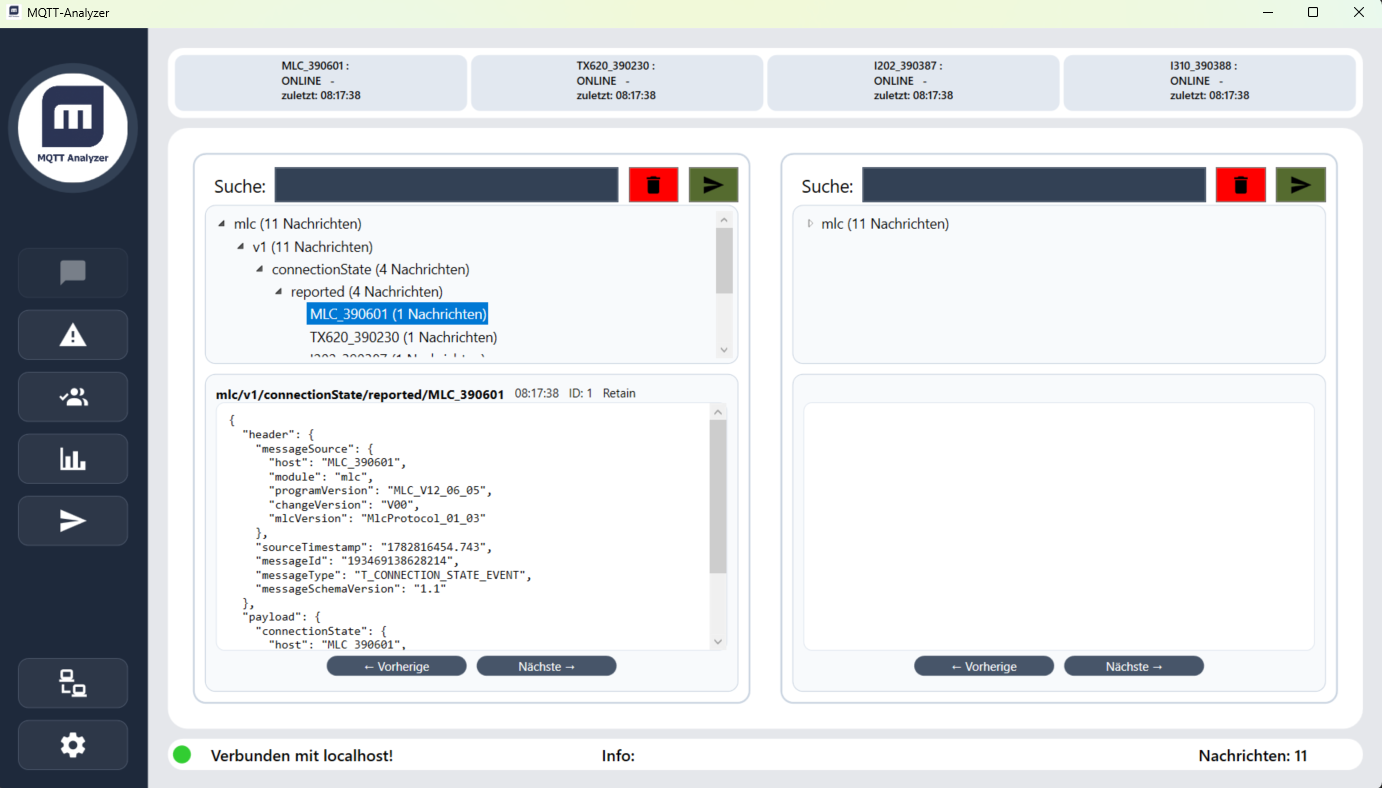
\includegraphics[width=0.6\textwidth]{images/MainWindow.png}
    \caption{Hauptansicht und Grundaufbau der Anwendung}
    \label{fig:MainWindow}
\end{figure}
\subsection{Nachrichtenansicht}
Die Nachrichtenansicht umfasst ein Dropdown-Menü, das ein Filtern der Nachrichten nach Topics ermöglicht. Zudem ist ein Suchfeld integriert, das eine manuelle Suche nach Begriffen in Payload, Topic oder Zeitstempel ermöglicht. Schließlich besteht die Möglichkeit, mittels eines Buttons die Nachrichten in eine Textdatei zu speichern. Darunter befindet sich eine Tabelle, in der die aus der Datenbank geladenen Nachrichten angezeigt werden.

Die Nachrichtenansicht verfügt über zwei unterschiedliche Einstellungen. Zunächst besteht die Möglichkeit, die Anzahl der gleichzeitig angezeigten Nachrichtenfenster zu konfigurieren. Diese können entweder ein, zwei oder vier Nachrichtenfenster umfassen (vgl. Abbildung \ref{fig:MessageViews}). Des Weiteren besteht die Möglichkeit, die Darstellung der Nachrichten zu konfigurieren. So kann eingestellt werden, ob die Payload lediglich bei Klick auf eine Nachricht angezeigt werden soll oder ob sie bei jeder Nachricht direkt angezeigt wird. Des Weiteren kann die Baumstruktur-Ansicht ausgewählt werden. Bei dieser werden die Topics automatisch nach ihrer Hierarchie in eine Baumstruktur umgewandelt, die man beliebig weit aufklappen kann. In XAML gibt es dafür ein UI-Element \lstinline{treeview}, das seine Daten aus der \texttt{ObservableCollection} \lstinline{FilteredTopics} bezieht (siehe \ref{lst:treeview}). Die Datenobjekte sind vom Typ \textit{TopicTreeNode}, während die Unterknoten aus der Eigenschaft \textit{Children} geladen werden. Die Erkennung und Speicherung der Topics in diesen Datenobjekten erfolgt durch die Methode \lstinline{AddTopicHierarchy(string topic)}) (siehe \ref{lst:AddTopicHierarchy}). Am Ende eines jeden Zweiges finden sich dann die neuesten Nachrichten dieses Topics wieder, die bei Klick in einem zusätzlichen Textfeld angezeigt werden können. Wurden unter dem ausgewählten Topic schon mehrere Nachrichten versendet, können durch zwei Buttons frühere und dann auch wieder spätere Nachrichten geladen und angezeigt werden. 

Die parallele Darstellung mehrerer Nachrichtenfenster erleichtert die Analyse verschiedener Kommunikationsströme erheblich. Gleichzeitig erhöht sich die Anzahl der Datenbankabfragen und Aktualisierungen der Benutzeroberfläche. Des Weiteren verbessert die hierarchische Darstellung der Topics durch die Baumstrukturdarstellung die Übersichtlichkeit komplexer MQTT-Strukturen erheblich. Gleichzeitig ist der Aufbau und die Pflege der Baumstruktur aufwendiger als die Darstellung in einer einfachen Tabelle. Bei sehr großen Topic-Hierarchien kann zudem die Navigationsgeschwindigkeit des Benutzers sinken. Diese Funktionen stellen somit einen Kompromiss zwischen Analysekomfort und Ressourcenverbrauch dar.

\begin{figure}[h]
    \centering
    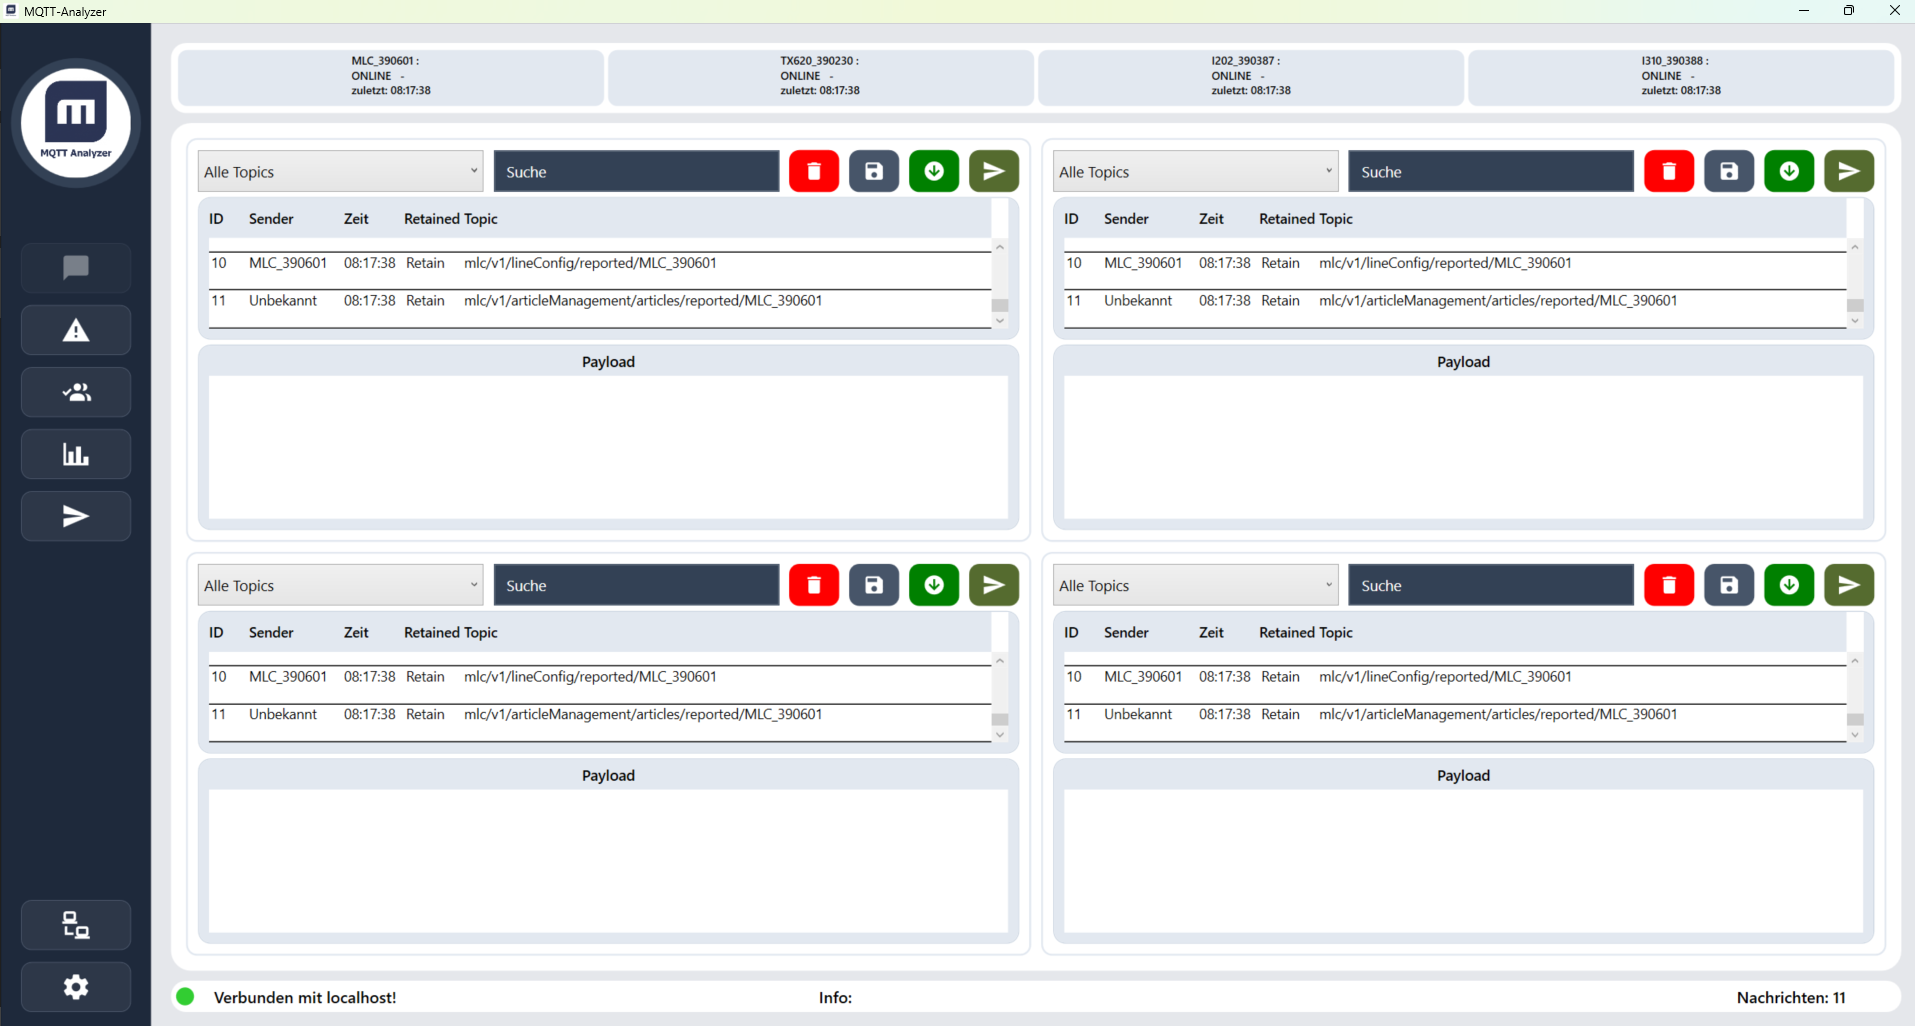
\includegraphics[width=0.8\textwidth]{images/MessageViews.png}
    \caption{Darstellung von 4 Nachrichtenfenstern gleichzeitig}
    \label{fig:MessageViews}
\end{figure}

Die simultane Präsentation mehrerer Nachrichtenfenster wird durch die Verwendung eines \lstinline|ItemsControl|-Elements realisiert. Das vorliegende Element weist ein Binding auf die Collection MessageViews auf, welche die aktuell anzuzeigenden Nachrichtenansichten enthält. Für jedes Objekt, das in der Collection enthalten ist, wird automatisch eine eigene Instanz der Nachrichtenansicht erzeugt. Die Anordnung der einzelnen Nachrichtenfenster wird über ein \lstinline|UniformGrid| festgelegt (vgl. Listing \ref{lst:UniformGrid})

\begin{lstlisting}[
    language=XML,
    caption={UniformGrid zur automatischen Platzierung von Objekten},
    label={lst:UniformGrid}
    ]
<UniformGrid Rows="{Binding Rows}"
 	Columns="{Binding Columns}" />
\end{lstlisting}

Dabei sind die Eigenschaften der Elemente ,,Row'' und ,,Column'' mit Variablen aus dem View-Model verknüpft. Durch die Anpassung der Stilvorlagen kann eine dynamische Veränderung des Layouts erzielt werden. Das \lstinline|UniformGrid| gewährleistet eine gleichmäßige Verteilung aller enthaltenen Elemente auf die verfügbaren Zeilen und Spalten.

Innerhalb des \lstinline|ItemTemplates| wird definiert, wie jedes Element der Collection dargestellt werden soll (vgl. Listing \ref{lst:ContentControl}).
\begin{lstlisting}[
    language=XML,
    caption={Aktivierung bzw. Deaktivierung der Navigationsbuttons},
    label={lst:ContentControl}
    ]
<DataTemplate>
    <Border Margin="5">
        <ContentControl Content="{Binding}" />
    </Border>
</DataTemplate>
\end{lstlisting}

Jedes Nachrichtenfenster wird zunächst von einer \lstinline|Border| umgeben. Innerhalb des definierten Rahmens befindet sich ein \lstinline|ContentControl|, dessen Inhalt direkt an das jeweilige Objekt in der Collection gebunden wird.

Infolge dessen besteht die Möglichkeit, eine beliebige Anzahl von Nachrichtenansichten in der \textit{Collection} zu speichern. Die Anzeige weist eine automatische Anpassung auf, die durch die im View-Model definierten Zeilen- und Spaltenvorgaben determiniert wird.
\subsection{Fehleransicht}
Die Fehleransicht besteht aus einem Dropdown-Menü, in dem die Fehler nach Struktur- und Automatisierungs-Ablauf-Fehler gefiltert werden können, und einer Tabelle, in der die Nachrichten mit Sender, Topic, Zeitstempel und der Fehlernachricht angezeigt werden. 

Durch einen Klick auf eine Fehlernachricht öffnet sich automatisch ein Nachrichtenfenster, in dem dann die Nachricht angezeigt wird. Es werden automatisch die 24 vorherigen und 25 nachkommenden Nachrichten aus der Datenbank mitgeladen und angezeigt, damit der Nachrichtenfluss rund um die Nachricht verstanden werden kann.
\subsection{Nachrichtenversand}
Der Reiter für den Nachrichtenversand teilt sich in zwei Hälften auf. Im oberen Teil können Topic, Header und Payload der Nachricht eingegeben werden und versendet werden. Braucht man die Nachricht oder das Nachrichtenformat öfter, kann der Nachricht ein Vorlagen-Name versehen werden und in der Datenbank gespeichert werden. In einer Liste mit allen abgespeicherten Nachrichtenvorlagen können diese ausgewählt werden. Daraufhin werden die entsprechenden Felder automatisch ausgefüllt. 

In der unteren Hälfte können selbst Buttons erstellt werden, die beim Klick eine hinterlegte Nachricht versenden. Für das Anlegen eines solchen Nachrichtenbuttons wird lediglich die eingegebene Nachrichtenvorlage durch einen Buttonklick als neues Buttonmodell gespeichert. Die Buttons platzieren sich dann automatisch mittels eines \lstinline|ItemsControl| (vgl. Listing \ref{lst:PublishButton}). Dieses wird mit der \textit{ObservableCollection} \lstinline|CustomButtons| verknüpft, in der die zuvor eingegebenen Informationen zu den verschiedenen Buttons gespeichert sind. Dadurch werden diese Informationen beim Klick auf den entsprechenden Button an die Methode \lstinline|PublishButtons| übergeben, wodurch die Nachricht versendet wird.

Die Daten des Buttons werden ebenfalls in der Datenbank gespeichert und werden beim Starten der Anwendung geladen, wodurch die Buttons wieder automatisch angezeigt werden. 

Die Speicherung von Vorlagen in einer Datenbank ermöglicht eine dauerhafte Bereitstellung über Programmstarts hinweg. Eine Speicherung in Konfigurationsdateien wäre ebenfalls möglich gewesen und hätte den Datenbankumfang reduziert. Aufgrund der einfacheren Verwaltung strukturierter Daten wurde jedoch die datenbankgestützte Lösung bevorzugt.
\subsection{Teilnehmerüberwachungsansicht}
Die Teilnehmerübersicht besteht aus zwei Bereichen: Oben können Diagramme für jeden einzelnen Teilnehmer angezeigt werden, in denen zum einen der Verbindungsverlauf und zum anderen die Omac-Zustände, in denen sich die Teilnehmer über die Zeit hinweg befanden, angezeigt werden (vgl. Abbildung \ref{fig:ParticipantView}). Neben den Diagrammen für die einzelnen Teilnehmer kann auch ein Diagramm für alle Teilnehmer dargestellt werden. In diesem wird für jeden Teilnehmer ein Balken erstellt, in dem der Omac-Zustand in Abhängigkeit von der Zeit dargestellt ist. Dadurch kann auf einen Blick erkannt werden, wann welche Maschine in welchem Zustand war. 

Unter diesem Bereich befindet sich eine visuelle Anzeige, ob alle Teilnehmer verbunden sind, und eine Auflistung der in den MQTT-Nachrichten verschickten Linienartikel.
\begin{figure}[h]
    \centering
    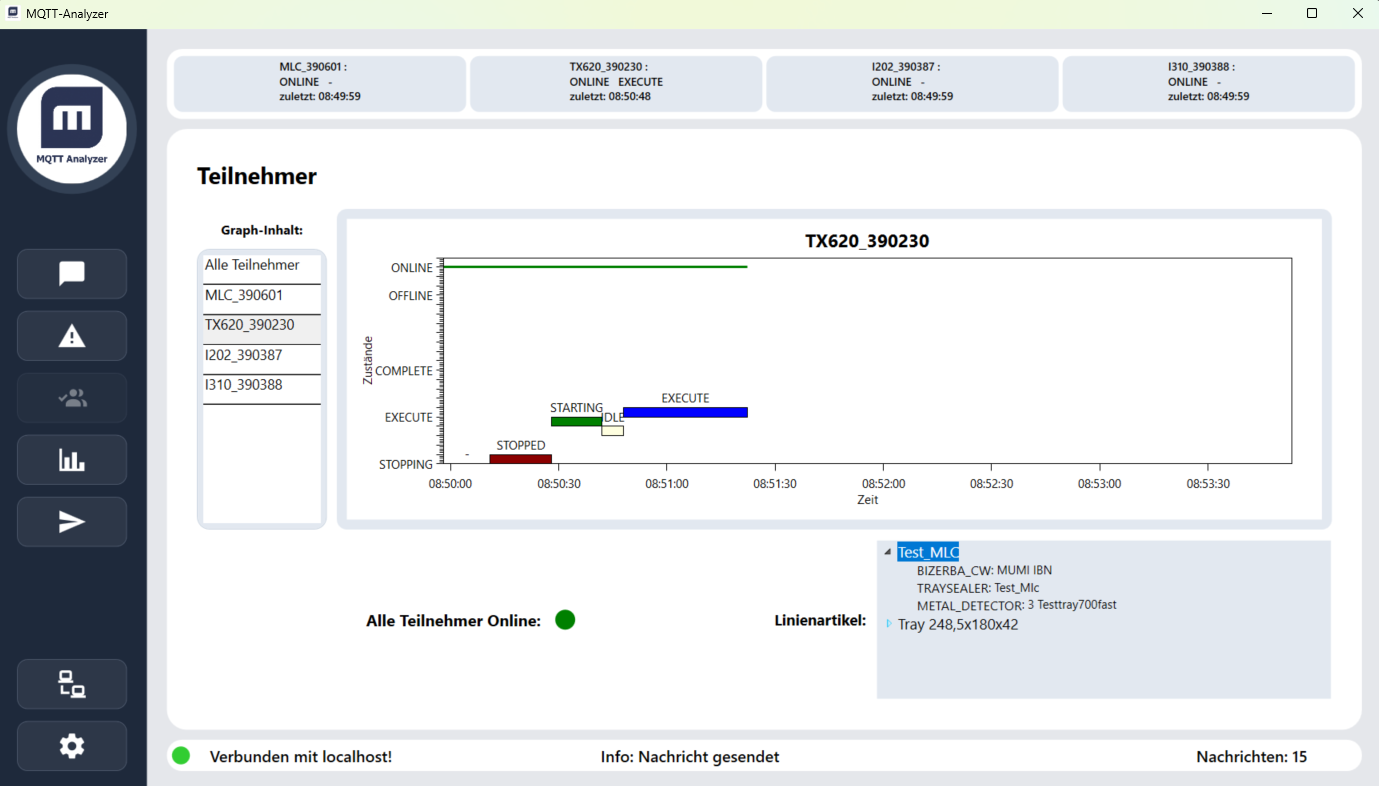
\includegraphics[width=0.8\textwidth]{images/ParticipantView.png}
    \caption{Teilnehmerüberwachungsansicht}
    \label{fig:ParticipantView}
\end{figure}
\subsection{Automatisierungs-Ablauf-Überwachungsansicht}
Die Ablauf-Überwachungsansicht besteht aus zwei Tabellen. Diese werden durch \texttt{DataGrids} in XAML erstellt und über \texttt{ObservableCollections} mit Daten aus dem View-Model verbunden. Die obere Tabelle stellt die gerade aktiven Abläufen mit erwarteten und eingetroffenen Nachrichten dar, während die untere die bereits abgeschlossenen Abläufe darstellt. Damit bei vielen Abläufen auch diese \texttt{ObservableCollection} nicht viel Arbeitsspeicher verbraucht, wird hier ähnlich zur Nachrichtendarstellung Paging verwendet. Dadurch werden immer nur 50 Abläufe in das \texttt{DataGrid} geladen. Ist der Anwender am Anfang oder Ende des \texttt{DataGrids} angekommen, werden die 10 weiteren Abläufe geladen, soweit diese vorhanden sind. Auch dieser Reiter verfügt über einen Button, mit dem ein automatisches Anzeigen der neuesten abgeschlossenen Abläufe ausgelöst wird.

\subsection{Einstellungen}
In den Einstellungen können mithilfe von Buttons verschiedene Parameter der Anwendung angepasst werden. Hierzu zählen die schon beschriebene Anzahl an dargestellten Nachrichtenfenstern, die Umstellung zwischen der kompakten Ansicht mit der Payload in einem zusätzlichen Feld oder der detaillierten Ansicht, bei der die Payload immer direkt bei der Nachricht steht. Des Weiteren lässt sich die Anzahl an geladenen und dargestellten Nachrichten in den Nachrichtenfenstern einstellen, wodurch der RAM-Verbrauch manuell gesteuert werden kann.

Die Konfiguration wird dauerhaft in einer SQLite-Datenbank gespeichert und beim Start der Anwendung automatisch geladen.

Zur Sicherstellung der am Anwender-Endgerät eingestellten IP-Adresse werden alle erkannten Netzwerk-Adapter mit eingestellter IP-Adresse zusätzlich unter den Einstellungen in einer Tabelle angezeigt. Dadurch kann jederzeit eingesehen werden, welche IP-Adresse gerade an welchem Netzwerk-Adapter eingestellt ist, ohne dafür die Einstellungen des Endgeräts aufrufen zu müssen.

Diese Funktion wird mithilfe der ,,System.Net''-Bibliothek implementiert, wobei die Adapter alle fünf Sekunden aktualisiert werden (vgl. Listing \ref{lst:NetworkAdapters}).
\begin{lstlisting}[
    language={[Sharp]C},
    caption={Erkennen der Netzwerk-Adapter und Adapter-Einstellungen},
    label={lst:NetworkAdapters}
    ]
while(true)
{ 
    NetworkAdapters?.Clear();
    foreach (NetworkInterface adapter in NetworkInterface.GetAllNetworkInterfaces())
    {
        var model = new NetworkAdapterModel();
        model.Name = adapter.Name;
        model.Status = adapter.OperationalStatus.ToString();
        var properties = adapter.GetIPProperties();
        foreach (var ip in properties.UnicastAddresses)
        {
            if (ip.Address.AddressFamily == AddressFamily.InterNetwork)
                model.Ip = ip.Address.ToString();
            if (ip.Address.AddressFamily == AddressFamily.InterNetworkV6)
                model.Ip = ip.Address.ToString();
        }
        NetworkAdapters?.Add(model);
    }
    await Task.Delay(5000);
}
\end{lstlisting}